\section{Results}\label{sec:results}

We organise the results around four questions: does learning beat classical adaptation for tracking (\ref{sec:rq1}), where does meta-learning add to it (\ref{sec:rq2}), what happens when a learned planner adapts inside the navigation stack (\ref{sec:rq3}), and how do methods behave beyond the training distribution (\ref{sec:rq4}).

\begin{table*}[t]
\centering
\caption{Tracking under new dynamics. A learned residual roughly halves the error of classical adaptation, and meta-learning helps most when it tunes the controller's gains. Held-out RMSE before and after adapting (mean, with the 95\% half-interval after adapting), OOD RMSE and OOD crash rate after adapting. Data: adaptation episodes used. Bold: best in column. Residual learners use \valSeedsRes\ training seeds, gain learners \valSeedsGain.}
\label{tab:tracking}
\footnotesize
% generated by figures_scripts/tracking_table.py; do not edit
\begin{tabular}{@{}llrrrrrrr@{}}
\toprule
 & & \multicolumn{4}{c}{Combination 1: residual on controller} & \multicolumn{3}{c}{Combination 2: controller gains} \\
\cmidrule(lr){3-6}\cmidrule(l){7-9}
Method & Data & Before & After & OOD & OOD crash & Before & After & OOD \\
 & (ep.) & (cm) & (cm) & (cm) & (\%) & (cm) & (cm) & (cm) \\
\midrule
\multicolumn{9}{@{}l}{\emph{Classical}} \\
Classical (nominal gains) & 0 & 21.4 & 21.4 & 78.7 & \textbf{34} & 21.4 & 21.4 & 78.7 \\
Classical + L1 & 0 & 15.5 & 15.5 & 72.1 & 52 & -- & -- & -- \\
\multicolumn{9}{@{}l}{\emph{Non-meta learned}} \\
DR (no adapt.) & 0 & \textbf{7.3} & \textbf{7.3} & \textbf{63.1} & 44 & 14.4 & 14.4 & 76.9 \\
DR + fine-tune & 30 & \textbf{7.3} & 8.0{\scriptsize$\pm$1.0} & 63.6 & 43 & 14.4 & 14.2{\scriptsize$\pm$1.9} & 75.5 \\
\multicolumn{9}{@{}l}{\emph{Gradient meta-learning}} \\
MAML & 30 & 8.7 & 7.8{\scriptsize$\pm$1.1} & 70.8 & 49 & 15.6 & 13.7{\scriptsize$\pm$2.7} & \textbf{69.8} \\
FOMAML & 30 & 8.5 & 7.8{\scriptsize$\pm$1.0} & 66.9 & 46 & 15.7 & 13.9{\scriptsize$\pm$2.8} & 72.6 \\
ANIL & 30 & 8.6 & 7.7{\scriptsize$\pm$1.1} & 70.4 & 49 & -- & -- & -- \\
Meta-SGD & 30 & 8.7 & 7.8{\scriptsize$\pm$1.1} & 69.3 & 48 & 15.6 & \textbf{11.3{\scriptsize$\pm$2.0}} & 69.9 \\
Reptile & 30 & 15.2 & 14.8{\scriptsize$\pm$2.0} & 68.6 & 36 & \textbf{13.5} & 13.4{\scriptsize$\pm$1.7} & 75.4 \\
\multicolumn{9}{@{}l}{\emph{Context meta-learning}} \\
PEARL & 3 & 10.5 & 9.0{\scriptsize$\pm$1.1} & 69.2 & 49 & -- & -- & -- \\
RL$^2$ & 3 & 18.4 & 17.4{\scriptsize$\pm$1.5} & 64.6 & 36 & -- & -- & -- \\
\bottomrule
\end{tabular}

\end{table*}

\begin{figure*}[t]
\centering
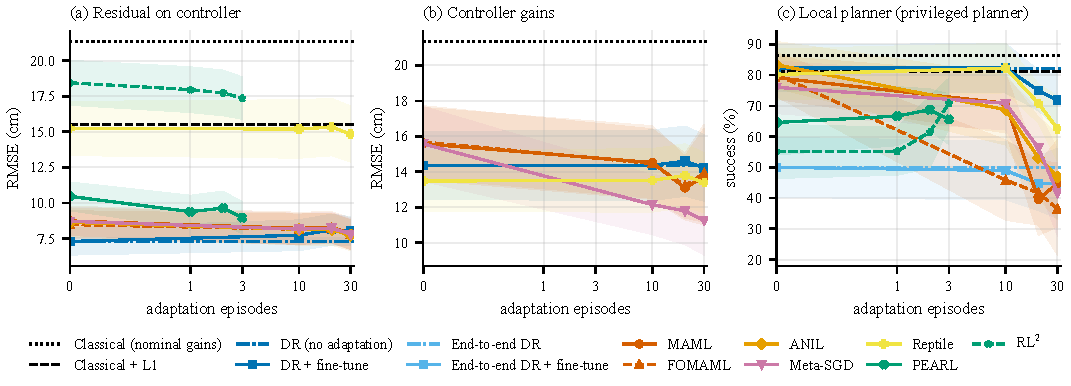
\includegraphics[width=\textwidth]{figures/adaptation_curves.pdf}
\caption{Adaptation pays off when it tunes classical gains (b), barely moves a learned residual (a), and at the meta-trained step size degrades learned navigation planners (c). Held-out tasks; mean and 95\% interval over tasks and seeds; horizontal lines are methods that do not adapt. A stage is one update from 10 episodes for the gradient-based methods and one more episode of experience for PEARL and RL$^2$. End-to-end planners are omitted from (c); see Table~\ref{tab:nav}.}
\label{fig:curves}
\end{figure*}

\subsection{Learning versus classical adaptation}\label{sec:rq1}

\textbf{A learned residual roughly halves the error of classical adaptation.} On held-out tasks the nominal geometric controller tracks with \valResClassicalPost\,cm RMSE and L1 augmentation with \valResLonePost\,cm (Table~\ref{tab:tracking}). A DR residual trained over all tasks reaches \valResDrPost\,cm without any adaptation. To make sure L1 is not a weak baseline, we grid-searched its predictor pole and filter bandwidth on training tasks (best: \valLoneTunedPole\,s$^{-1}$, \valLoneTunedCutoff\,rad/s); tuning lowers its held-out error only from \valLoneDefaultTest\ to \valLoneTunedTest\,cm on a common set of episodes, still about twice the residual's.

\subsection{Where meta-learning adds value}\label{sec:rq2}

\textbf{On top of a residual, meta-learning adds little.} MAML, FOMAML, ANIL and Meta-SGD start slightly worse than DR (\valResMamlPre, \valResFomamlPre, \valResAnilPre\ and \valResMetasgdPre\,cm) and improve with 30 adaptation episodes to \valResMamlPost, \valResFomamlPost, \valResAnilPost\ and \valResMetasgdPost\,cm, within the interval of DR's \valResDrPost\,cm (Fig.~\ref{fig:curves}a). With the same training budget as DR (Sec.~\ref{sec:learners}), they end where DR starts. Fine-tuning DR with PPO makes it slightly worse (\valResDrftPost\,cm), and Reptile trails at \valResReptilePost\,cm. Of the context-based methods, PEARL adapts from far less data (\valResPearlPre\ to \valResPearlPost\,cm with three episodes of context) but does not reach the gradient methods; RL$^2$ is the weakest learned residual (\valResRltwoPost\,cm).

\textbf{Adapting the classical gains is where meta-learning pays off.} When the policy chooses the controller's seven gains (Combination 2), every MAML-family method improves markedly with adaptation: Meta-SGD from \valGainMetasgdPre\ to \valGainMetasgdPost\,cm, MAML to \valGainMamlPost\,cm and FOMAML to \valGainFomamlPost\,cm, while gains tuned by DR stay at \valGainDrPost\,cm, or \valGainDrftPost\,cm with fine-tuning (Fig.~\ref{fig:curves}b). Paired over the same \valGainPairedN\ task--seed combinations, Meta-SGD improves on fine-tuned DR gains by \valGainPairedDiff\,cm (95\% bootstrap interval \valGainPairedLo--\valGainPairedHi\,cm) and wins on \valGainPairedWin\% of pairs. Adapted gains remain above the learned residual's error, but a seven-dimensional gain vector is a far smaller, more interpretable and more easily bounded object to adapt on a real vehicle.

\subsection{Adaptation inside the navigation stack}\label{sec:rq3}

\begin{table*}[t]
\centering
\caption{Navigation in unseen rooms. The classical local planner is the most reliable on the full stack, and gradient-based adaptation at the meta-trained step size lowers learned planners' success. Success and collision rates before and after adapting, with the privileged planner (3 stages) and on the full online-mapping stack (1 stage), and OOD success. \valSeedsNav\ training seeds; each episode in its own unseen room. Bold: best in column.}
\label{tab:nav}
\footnotesize
% generated by figures_scripts/navigation_table.py; do not edit
\begin{tabular}{@{}llrrrrrrr@{}}
\toprule
 & & \multicolumn{3}{c}{Privileged planner (96 rooms)} & \multicolumn{3}{c}{Full stack (48 rooms)} & OOD \\
\cmidrule(lr){3-5}\cmidrule(lr){6-8}
Method & Data & Before & After & Coll. & Before & After & Coll. & After \\
 & (ep.) & (\%) & (\%) & (\%) & (\%) & (\%) & (\%) & (\%) \\
\midrule
\multicolumn{9}{@{}l}{\emph{Classical}} \\
Classical (nominal gains) & 0 & \textbf{83} & \textbf{83} & \textbf{14} & \textbf{73} & \textbf{73} & \textbf{7} & 16 \\
Classical + L1 & 0 & 77 & 77 & 21 & \textbf{73} & \textbf{73} & 9 & 8 \\
\multicolumn{9}{@{}l}{\emph{Non-meta learned}} \\
DR (no adaptation) & 0 & 72 & 72 & 28 & 44 & 44 & 56 & 13 \\
DR + fine-tune & 30 & 72 & 71 & 29 & 44 & 50 & 50 & \textbf{17} \\
End-to-end DR & 0 & 52 & 52 & 48 & 51 & 51 & 49 & 10 \\
End-to-end DR + fine-tune & 30 & 52 & 46 & 54 & 51 & 47 & 53 & 16 \\
\multicolumn{9}{@{}l}{\emph{Gradient meta-learning (warm-started)}} \\
MAML & 30 & 73 & 36 & 60 & 46 & 32 & 67 & 8 \\
FOMAML & 30 & 76 & 31 & 69 & 53 & 31 & 69 & 5 \\
ANIL & 30 & 76 & 35 & 65 & 49 & 45 & 55 & 8 \\
Meta-SGD & 30 & 71 & 49 & 50 & 46 & 48 & 51 & 6 \\
Reptile & 30 & 72 & 71 & 29 & 46 & 47 & 53 & 14 \\
\multicolumn{9}{@{}l}{\emph{Context meta-learning (from scratch)}} \\
PEARL & 3 & 70 & 71 & 26 & 50 & 55 & 42 & 9 \\
RL$^2$ & 3 & 60 & 55 & 45 & 34 & 39 & 60 & 8 \\
\bottomrule
\end{tabular}

\end{table*}

\textbf{Gradient-based adaptation degrades learned planners at the meta-trained step size.} With the privileged planner, the warm-started MAML-family planners lose success as they adapt: MAML from \valNavMamlPre\% to \valNavMamlPost\%, FOMAML from \valNavFomamlPre\% to \valNavFomamlPost\%, ANIL from \valNavAnilPre\% to \valNavAnilPost\% and Meta-SGD from \valNavMetasgdPre\% to \valNavMetasgdPost\% (Table~\ref{tab:nav}, Fig.~\ref{fig:curves}c), with collisions rising as success falls. The decline already appears after the single update they were meta-trained for (MAML: \valNavMamlStageOne\%), so it is not only extrapolation. Methods that adapt conservatively stay flat: Reptile (\valNavReptilePre\% to \valNavReptilePost\%) and DR with fine-tuning (\valNavDrftPre\% to \valNavDrftPost\%) take small Adam steps, and PEARL (\valNavPearlPre\% to \valNavPearlPost\%) takes none. RL$^2$ does not improve with experience (\valNavRltwoPre\% to \valNavRltwoPost\%).

\begin{table}[t]
\centering
\caption{The navigation decline is a step-size effect. Success by adaptation stage and final collision rate with the inner step scaled from its meta-trained value, or with 30 instead of 10 episodes per update. Privileged planner, 16 held-out tasks in unseen rooms, seed-0 checkpoints.}
\label{tab:stepsize}
\footnotesize
% generated by figures_scripts/step_size_table.py; do not edit
\begin{tabular}{@{}lrrrrr@{}}
\toprule
 & \multicolumn{4}{c}{Success by stage (\%)} & Coll. \\
\cmidrule(lr){2-5}
Configuration & 0 & 1 & 2 & 3 & (\%) \\
\midrule
MAML, meta-trained step & 69 & 58 & 39 & 25 & 69 \\
MAML, step $\times$0.3 & 69 & 75 & 64 & 66 & 34 \\
MAML, step $\times$0.1 & 69 & 72 & 70 & 72 & 28 \\
MAML, 30 ep./stage & 69 & 75 & 62 & 64 & 36 \\
Meta-SGD, learned steps & 67 & 64 & 50 & 38 & 58 \\
Meta-SGD, steps $\times$0.3 & 67 & 69 & 67 & 73 & 27 \\
Meta-SGD, steps $\times$0.1 & 67 & 70 & 69 & 70 & 30 \\
\bottomrule
\end{tabular}

\end{table}

\textbf{The decline is a step-size and data-budget effect.} Scaling the inner step at test time (Table~\ref{tab:stepsize}) shows that the drop occurs at the meta-trained step with 10 episodes per update (MAML: \valStepMamlOnePre\% to \valStepMamlOnePost\%). With a 10$\times$ smaller step MAML holds at \valStepMamlTenthPost\% (Meta-SGD: \valStepMetasgdTenthPost\%), and with three times more episodes per update at the original step it holds at \valStepMamlDataPost\%. Smaller steps prevent the damage but buy little: success stays within a few points of its pre-adaptation level. Step sizes meta-learned for one task family therefore do not transfer to the sparse, high-variance returns of navigation, and on a real vehicle they should be scaled down or paired with more data per update.

\textbf{On the full stack, the classical planner is the most reliable.} With a map built in flight and A* replanning, the classical local planner reaches the goal in \valNavClassicalFullPost\% of \valNavFullFlights\ flights in unseen rooms with \valNavClassicalFullColl\% collisions, and L1 augmentation does not change this (\valNavClassicalloneFullPost\%). The learned planners reach \valNavFullLearnedLo--\valNavFullLearnedHi\% with \valNavFullCollLo--\valNavFullCollHi\% collisions. Learned planners also lose far more than the classical planner when the privileged planner is replaced by the online map (DR: \valNavDrPre\% to \valNavDrFullPost\%; classical: \valNavClassicalPre\% to \valNavClassicalFullPost\%). They were trained against carrots from a perfect map, and the online map's late-discovered obstacles and replanned paths fall outside that training distribution. Fig.~\ref{fig:flight} shows a recorded classical flight.

\textbf{The planner helps a learned policy only when the map is good.} With the privileged planner, the DR planner that follows the carrot beats the end-to-end DR planner that sees only the goal direction (\valNavDrPre\% vs \valNavEtoePre\%). On the full stack the order flips (\valNavDrFullPost\% vs \valNavEtoeFullPost\%): the end-to-end planner never depended on a map, so it loses nothing when the map is imperfect.

\begin{figure}[t]
\centering
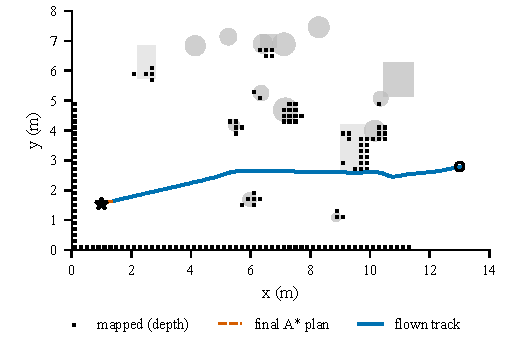
\includegraphics[width=\columnwidth]{figures/example_flights.pdf}
\caption{The classical stack maps an unseen room from its depth camera and reaches the goal. Grey: true obstacles (paler boxes hang overhead and are flown under); black: voxels mapped by the end of the flight; dashed: final A* plan; blue: flown track from start (circle) to goal (star).}
\label{fig:flight}
\end{figure}

\subsection{Beyond the training distribution}\label{sec:rq4}

\textbf{Every method fails out of distribution, and learned residuals crash more.} On the OOD tasks, which combine heavier payload, weaker motors, stronger wind and longer latency, no tracking method gets below \valOodRmseMin\,cm RMSE and no navigation method exceeds \valNavOodMax\% success. Learned residuals crash in \valResOodCrashLearnedLo--\valResOodCrashLearnedHi\% of OOD episodes, against \valResClassicalOodCrash\% for the nominal controller, and three adaptation stages change OOD error by at most \valOodAdaptMaxDelta\,cm. The pattern already appears just outside the training ranges: on a milder split that exceeds each range only slightly, the DR residual still tracks better than the nominal controller (\valMildDrRmse\ vs \valMildClassicalRmse\,cm), but DR and MAML-family residuals crash in \valMildResidCrashLo--\valMildResidCrashHi\% of episodes against \valMildClassicalCrash\%. Learned residuals thus trade safety margin for accuracy at the edge of the envelope, and the plain classical controller degrades most gracefully.
